\section{The setting}

\begin{frame}\frametitle{\secname}
    
\underline{Data:}

observations: $\big\{ \vec{x}^{(\alpha)} \big\}, \alpha = 1, \ldots, p; \quad \vec{x} \in \R^N$

$$
\vec x = \rmat{
x_1\\
x_2\\
\vdots\;\,\\
x_N
}
$$

Our entire dataset:
\[
\vec X = 
\left(
\begin{array}{cccc}
\Big| & \Big| & &\Big| \\[3mm]
\vec x^{(1)} & \vec x^{(2)} & \cdots &\vec x^{(p)}\\[2mm]
\Big| & \Big| & &\Big|
\end{array}
\right) \in \R^{N \times p}
\]

\end{frame}

\section{Dimensionality Reduction}

\begin{frame}\frametitle{\secname}
We want to reduce the number of elements in $\vec x \in \R^N$
while retaining as most of the intrinsic information content.

\question{For what purpose?}

\question{What is the difference between dimensionality reduction and compression, if any?}

\end{frame}

%\newpage
\subsection{Simple truncation}
\begin{frame}\frametitle{\subsecname}

Let\\[0.2cm]
$\vec x \in \R^N$,\\
$\E[\vec x] = \vec 0$ (i.e. for each variable $x_i$ its mean $m_i = \sum_{\alpha=1}^{p} x_i^{(\alpha)} = 0$) and $1 < M\, < N$.\\[0.2cm]
We simply transmit the first $M$ elements of $\vec x$. The recipient reconstructs all $N$ elements by adding zero entries for all missing elements (i.e. \textit{zero-padding}).\\[0.2cm]
How much error will they accumulate in this case?\\[0.2cm]
Let $\widetilde{\vec{x}}$ be the reconstructed observation. The first $M$ elements were transmitted perfectly, zero padding is used to extend the vector to its original size of $N$ elements:
\begin{align*}
MSE  &=  \frac{1}{p} \sum\limits_{\alpha = 1}^p ( \vec{x}^{(\alpha)} - \widetilde{\vec{x}}^{(\alpha)} )^2\\
     &=  \frac{1}{p} \sum\limits_{\alpha = 1}^p \left(\underbrace{\sum\limits_{j = 1}^M ( x_j^{(\alpha)} - \widetilde{x_j}^{(\alpha)} )^2}_{\substack{=0 \\\text{ (perfect transmission)}}} + \sum\limits_{j = M+1}^N ( x_j^{(\alpha)} - \underbrace{\widetilde{x_j}^{(\alpha)}}_{\substack{=0\\ \text{padded}}}\;)^2 \right)\\
     &=  \frac{1}{p} \sum\limits_{\alpha = 1}^p \sum\limits_{j = M+1}^N ( x_j^{(\alpha)} )^2 \\
     &=  \sum\limits_{j = M+1}^N \frac{1}{p} \sum\limits_{\alpha = 1}^p  ( x_j^{(\alpha)} )^2 \\
     &=  \sum\limits_{j = M+1}^N \sigma_j^2 \\
\end{align*}
They will end up with an MSE equal to $\sum_{j=M+1}^{N} \sigma_j^2$, where $\sigma_j^2$ is the variance of the $x_j$.\\

\underline{Objective:} Rotate/Transform the data s.t. truncating the transformed vector $\vec v \in \R^M$ is optimum in the sense of minimal MSE.

\end{frame}

\begin{frame}
    
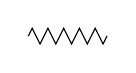
\begin{tikzpicture}
  %\draw [distance=5.4pt, postaction={decorate, draw=black, decoration=zigzag}] (0,0) -- (40pt,0);
\draw[decoration = {zigzag,segment length = 2mm, amplitude = 1mm},decorate] (0,0)--(1,0);
\end{tikzpicture}

% Please add the following required packages to your document preamble:
% \usepackage{graphicx}
\begin{table}[]
\resizebox{.5\textwidth}{!}{%
\begin{tabular}{|c|c|c|}
\cline{1-1} \cline{3-3}
Class & \hspace{.2\linewidth} & l\_2 \\ \cline{1-1} \cline{3-3} 
1 &  & -1 \\ \cline{1-1} \cline{3-3} 
2 &  & 1 \\ \cline{1-1} \cline{3-3} 
3 &  & 1 \\ \cline{1-1} \cline{3-3} 
\hspace{-9.55mm}
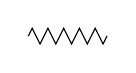
\begin{tikzpicture}
\draw[decoration={zigzag,segment length=2mm, amplitude=1mm},decorate](0,0)--(1.,0);
\end{tikzpicture}\hspace{-8.15mm} &  & -1 \\ \cline{1-1} \cline{3-3} 
\end{tabular}%
}
\end{table}

\end{frame}
